% SPDX-License-Identifier: BSD-2-Clause
%
% Copyright (C) 2026 embedded brains GmbH & Co. KG
%
% Redistribution and use in source and binary forms, with or without
% modification, are permitted provided that the following conditions
% are met:
% 1. Redistributions of source code must retain the above copyright
%    notice, this list of conditions and the following disclaimer.
% 2. Redistributions in binary form must reproduce the above copyright
%    notice, this list of conditions and the following disclaimer in the
%    documentation and/or other materials provided with the distribution.
%
% THIS SOFTWARE IS PROVIDED BY THE COPYRIGHT HOLDERS AND CONTRIBUTORS "AS IS"
% AND ANY EXPRESS OR IMPLIED WARRANTIES, INCLUDING, BUT NOT LIMITED TO, THE
% IMPLIED WARRANTIES OF MERCHANTABILITY AND FITNESS FOR A PARTICULAR PURPOSE
% ARE DISCLAIMED. IN NO EVENT SHALL THE COPYRIGHT OWNER OR CONTRIBUTORS BE
% LIABLE FOR ANY DIRECT, INDIRECT, INCIDENTAL, SPECIAL, EXEMPLARY, OR
% CONSEQUENTIAL DAMAGES (INCLUDING, BUT NOT LIMITED TO, PROCUREMENT OF
% SUBSTITUTE GOODS OR SERVICES; LOSS OF USE, DATA, OR PROFITS; OR BUSINESS
% INTERRUPTION) HOWEVER CAUSED AND ON ANY THEORY OF LIABILITY, WHETHER IN
% CONTRACT, STRICT LIABILITY, OR TORT (INCLUDING NEGLIGENCE OR OTHERWISE)
% ARISING IN ANY WAY OUT OF THE USE OF THIS SOFTWARE, EVEN IF ADVISED OF THE
% POSSIBILITY OF SUCH DAMAGE.

\documentclass[tikz,border=4pt]{standalone}
\usepackage[T1]{fontenc}
\usepackage[scaled]{helvet}
\renewcommand{\familydefault}{\sfdefault}
\usetikzlibrary{arrows.meta,positioning,fit,backgrounds,shapes.geometric}
\definecolor{ebblue}{HTML}{1F4E79}
\definecolor{boxfill}{HTML}{EAF1F8}
\definecolor{codefill}{HTML}{FFF4E0}
\definecolor{codeline}{HTML}{9C6500}
\definecolor{groupfill}{HTML}{F5F5F5}
\definecolor{flow}{HTML}{404040}
\newcommand{\code}[1]{{\ttfamily\scriptsize #1}}
\begin{document}
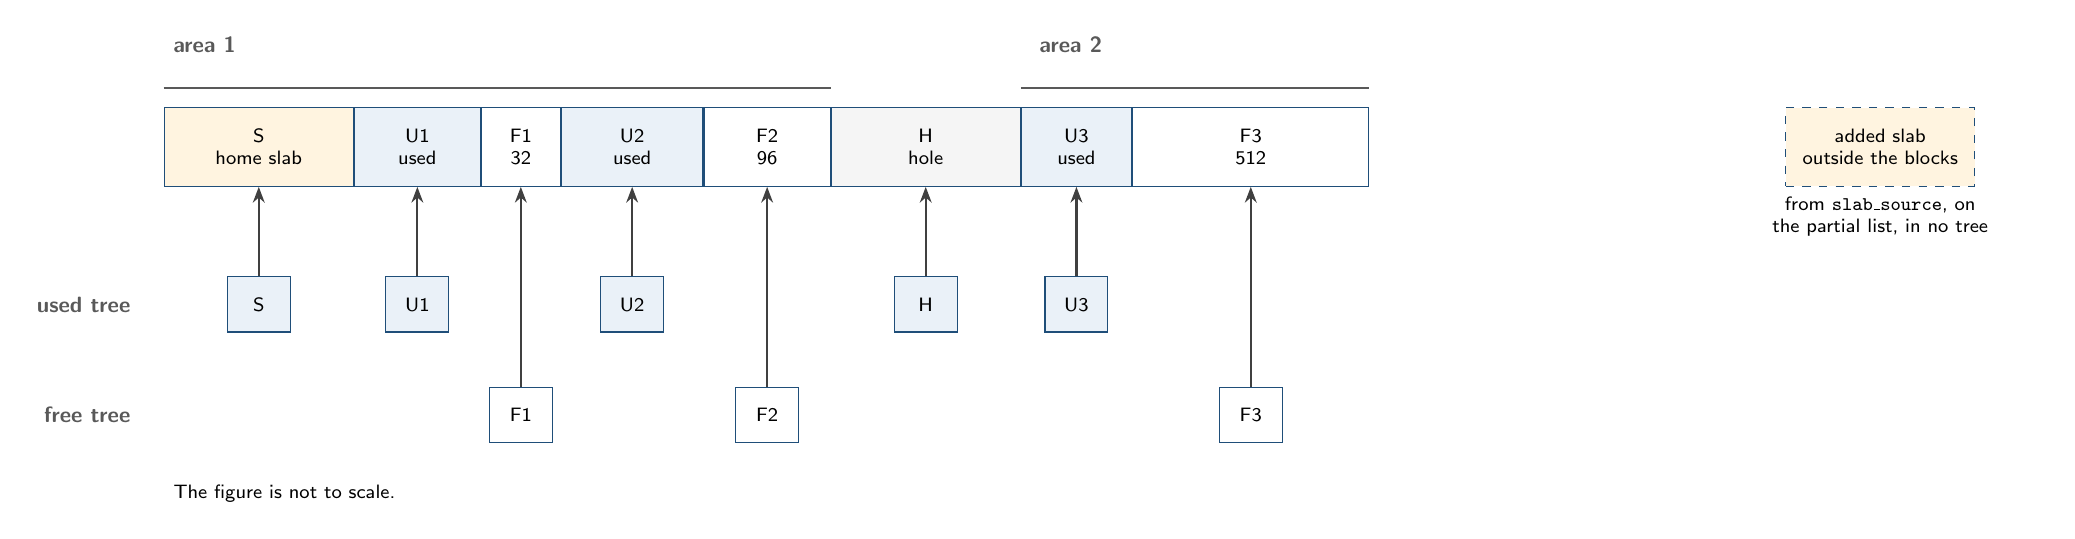
\begin{tikzpicture}[
    font=\small,
    blk/.style={draw=ebblue, minimum height=10mm, align=center,
      font=\scriptsize, inner sep=1pt},
    usedb/.style={blk, fill=boxfill},
    freeb/.style={blk, fill=white},
    slabb/.style={blk, fill=codefill},
    holeb/.style={blk, fill=groupfill},
    tag/.style={font=\scriptsize, align=center},
    title/.style={font=\footnotesize\bfseries, text=gray!70!black},
    arr/.style={-{Stealth[length=2mm]}, thick, draw=flow}]
  \node[title, anchor=west] at (0,1.3) {area 1};
  \node[title, anchor=west] at (11.0,1.3) {area 2};
  \node[slabb, minimum width=24mm, anchor=west] (S) at (0,0) {S\\home slab};
  \node[usedb, minimum width=16mm, anchor=west] (U1) at (S.east) {U1\\used};
  \node[freeb, minimum width=10mm, anchor=west] (F1) at (U1.east) {F1\\32};
  \node[usedb, minimum width=18mm, anchor=west] (U2) at (F1.east) {U2\\used};
  \node[freeb, minimum width=16mm, anchor=west] (F2) at (U2.east) {F2\\96};
  \node[holeb, minimum width=24mm, anchor=west] (H) at (F2.east) {H\\hole};
  \node[usedb, minimum width=14mm, anchor=west] (U3) at (H.east) {U3\\used};
  \node[freeb, minimum width=30mm, anchor=west] (F3) at (U3.east) {F3\\512};
  \draw[thick, draw=gray!70!black] (0,0.75) -- (F2.north east |- 0,0.75);
  \draw[thick, draw=gray!70!black] (U3.north west |- 0,0.75) -- (F3.north east |- 0,0.75);
  % Descriptors of the used tree and the free tree
  \node[title, anchor=east] at (-0.3,-2.0) {used tree};
  \node[title, anchor=east] at (-0.3,-3.4) {free tree};
  \foreach \b in {S, U1, U2, H, U3} {
    \node[usedb, minimum width=8mm, minimum height=7mm] (d\b) at (\b |- 0,-2.0) {\b};
    \draw[arr] (d\b) -- (\b.south);
  }
  \foreach \b in {F1, F2, F3} {
    \node[freeb, minimum width=8mm, minimum height=7mm] (d\b) at (\b |- 0,-3.4) {\b};
    \draw[arr] (d\b) -- (\b.south);
  }
  \node[tag, anchor=west] at (0,-4.4) {The figure is not to scale.};
  \node[slabb, minimum width=24mm, dashed] (A) at (21.8,0) {added slab\\outside the blocks};
  \node[tag, anchor=north, text width=40mm] at (A.south) {from \code{slab\_source}, on the partial list, in no tree};
\end{tikzpicture}
\end{document}
